% $Id: oscarpkg-howto.tex,v 1.10 2003/10/01 20:36:37 naughtont Exp $
%
% * Sun Jul 27 2003  11:11:44AM    Thomas Naughton  <naughtont@ornl.gov>
% - Initial creation for distribution to OSCAR and SSS community to assist
%   with creation of new OSCAR Packages.  Ultimately this should be merged 
%   with the "OSCAR Architecture" document, but for now I'm just trying to
%   get something out.
% - I am pooling together information from the arch doc as well as some
%   existing text from previous papers, specifically OLS'03.  
% 
% $COPYRIGHT$
%      
\documentclass[letterpaper]{article}

% -*- latex -*-
%
% $Id: defs.tex,v 1.6 2002/06/12 06:46:56 jsquyres Exp $
%
% $COPYRIGHT$
%

\usepackage{times}
\usepackage{graphicx}
\usepackage{fullpage}

% Versions

\include{version}

% Image Scaling
\def\imgscale{0.75}

% PDF stuff
 
\newif\ifpdf
\ifx\pdfoutput\undefined
   \pdffalse
\else
   \pdfoutput=1
   \pdftrue
\fi
 
\setcounter{tocdepth}{3}
 
\ifpdf
  \usepackage[pdftex,
              colorlinks=true,
              linkcolor=blue,filecolor=blue,pagecolor=blue,urlcolor=blue
              ]{hyperref}
  \def\figext{png}
  \def\sbsext{png}
  \newcommand{\xref}[2]{\hyperref[#1]{#2}}
  \newcommand{\mailto}[1]{\href{mailto:#1}{#1}}
\else
  \def\figext{eps}
  \def\sbsext{eps}
  \newcommand{\xref}[2]{#2}
  \newcommand{\href}[2]{\underline{#2}}
  \newcommand{\url}[1]{\href{#1}{#1}}
  \newcommand{\mailto}[1]{\href{#1}{#1}}
\fi

\newcommand{\email}[1]{\href{#1}{#1}}

% Stoopid European-based Linux distributions...
% Gotta force letter size paper, not A4

\ExecuteOptions{letterpaper}

% Discussion item; stolen from the MPI standard

\newenvironment{discuss}{\begin{list}{}{}\item[]{\it Discussion item:}
\addcontentsline{toc}{subsection}{Discussion Item}
}{{\rm ({\it End of discussion item.})} \end{list}}

% Rationale item; stolen from the MPI standard

\newenvironment{rationale}{\begin{list}{}{}\item[]{\it Rationale.}
}{{\rm ({\it End of rationale.})} \end{list}}

% Stolen from the MPI standard

\newcommand{\cmd}[1]{\texttt{#1}}
\newcommand{\odrcat}[1]{\textsf{#1}}
\newcommand{\odrkey}[1]{\texttt{#1}}
\newcommand{\file}[1]{\texttt{#1}}
\newcommand{\rpmname}[1]{\texttt{#1}}
\newcommand{\user}[1]{\texttt{#1}}

\newcommand{\term}[1]{\textit{#1}}

\newcommand{\msg}[1]{\textbf{#1}}
\newcommand{\msgout}[1]{\textbf{\texttt{#1}}}

\newcommand{\panel}[1]{\textbf{\texttt{#1}}}
\newcommand{\button}[1]{\textbf{\texttt{#1}}}
\newcommand{\field}[1]{\textit{\texttt{#1}}}

% Also stolen from the MPI standard
% intended for general change marks not associated with a certain version
\def\begchange{\marginpar[\hspace*{-60pt}\mbox{\hspace*{10pt}
$\top$ \tiny (General)}]{\mbox{$\top$ \tiny (General)}}}
\def\endchange{\marginpar[\hspace*{-60pt}\mbox{\hspace*{10pt}
$\bot$ \tiny (General)}]{\mbox{$\bot$ \tiny (General)}}}
%get rid of these change marks
%\def\begchange{}
%\def\endchange{}


\title{HOWTO: Create an OSCAR Package}
\author{Core OSCAR Team}

\begin{document}
\maketitle

% Comment out the Draft line once the paper is finished.
\begin{center}
  {\catcode`\$=11\tiny\noindent Draft $Id: oscarpkg-howto.tex,v 1.10 2003/10/01 20:36:37 naughtont Exp $}
\end{center}

%-------------------------------------------------------------
% Generate Table Of Contents 
%-------------------------------------------------------------
\tableofcontents

\newpage


%-------------------------------------------------------------
% Section: Introduction 
%-------------------------------------------------------------
% -*- latex -*-
%
% $Id: intro.tex,v 1.1 2001/12/13 17:30:48 mchasal Exp $
%
% $COPYRIGHT$
%

\documentclass[letterpaper,11pt]{article}

% -*- latex -*-
%
% $Id: defs.tex,v 1.6 2002/06/12 06:46:56 jsquyres Exp $
%
% $COPYRIGHT$
%

\usepackage{times}
\usepackage{graphicx}
\usepackage{fullpage}

% Versions

\include{version}

% Image Scaling
\def\imgscale{0.75}

% PDF stuff
 
\newif\ifpdf
\ifx\pdfoutput\undefined
   \pdffalse
\else
   \pdfoutput=1
   \pdftrue
\fi
 
\setcounter{tocdepth}{3}
 
\ifpdf
  \usepackage[pdftex,
              colorlinks=true,
              linkcolor=blue,filecolor=blue,pagecolor=blue,urlcolor=blue
              ]{hyperref}
  \def\figext{png}
  \def\sbsext{png}
  \newcommand{\xref}[2]{\hyperref[#1]{#2}}
  \newcommand{\mailto}[1]{\href{mailto:#1}{#1}}
\else
  \def\figext{eps}
  \def\sbsext{eps}
  \newcommand{\xref}[2]{#2}
  \newcommand{\href}[2]{\underline{#2}}
  \newcommand{\url}[1]{\href{#1}{#1}}
  \newcommand{\mailto}[1]{\href{#1}{#1}}
\fi

\newcommand{\email}[1]{\href{#1}{#1}}

% Stoopid European-based Linux distributions...
% Gotta force letter size paper, not A4

\ExecuteOptions{letterpaper}

% Discussion item; stolen from the MPI standard

\newenvironment{discuss}{\begin{list}{}{}\item[]{\it Discussion item:}
\addcontentsline{toc}{subsection}{Discussion Item}
}{{\rm ({\it End of discussion item.})} \end{list}}

% Rationale item; stolen from the MPI standard

\newenvironment{rationale}{\begin{list}{}{}\item[]{\it Rationale.}
}{{\rm ({\it End of rationale.})} \end{list}}

% Stolen from the MPI standard

\newcommand{\cmd}[1]{\texttt{#1}}
\newcommand{\odrcat}[1]{\textsf{#1}}
\newcommand{\odrkey}[1]{\texttt{#1}}
\newcommand{\file}[1]{\texttt{#1}}
\newcommand{\rpmname}[1]{\texttt{#1}}
\newcommand{\user}[1]{\texttt{#1}}

\newcommand{\term}[1]{\textit{#1}}

\newcommand{\msg}[1]{\textbf{#1}}
\newcommand{\msgout}[1]{\textbf{\texttt{#1}}}

\newcommand{\panel}[1]{\textbf{\texttt{#1}}}
\newcommand{\button}[1]{\textbf{\texttt{#1}}}
\newcommand{\field}[1]{\textit{\texttt{#1}}}

% Also stolen from the MPI standard
% intended for general change marks not associated with a certain version
\def\begchange{\marginpar[\hspace*{-60pt}\mbox{\hspace*{10pt}
$\top$ \tiny (General)}]{\mbox{$\top$ \tiny (General)}}}
\def\endchange{\marginpar[\hspace*{-60pt}\mbox{\hspace*{10pt}
$\bot$ \tiny (General)}]{\mbox{$\bot$ \tiny (General)}}}
%get rid of these change marks
%\def\begchange{}
%\def\endchange{}


\begin{document}

\title{OSCAR: A packaged Cluster software stack for \\
       High Performance Computing} 
\author{The Open Cluster Group \\
\url{http://www.openclutergroup.org/}}

\date{December 13, 2001}

\maketitle

\abstract{OSCAR is a fully integrated easy to install bundle of
software designed to make it easy to build and use a cluster for high
performance computing.  Everything you need to build, maintain, and
use a modest sized Linux cluster is included in OSCAR.  In this note,
we introduce OSCAR and provide the background information you need to
use it.}


\section{Introduction}
OSCAR is a package of RPM's, perl-scripts, libraries, tools, and
whatever else is needed to build and use a modest-sized Linux cluster.
With OSCAR, you don't need to roam the web to find what you need.
Just download a single package, install it, and you're ready to start
using your cluster.

The acronym, OSCAR, is a bit contrived, but it goes a long way towards
explaining what the goal of the OSCAR project is: 
\begin{center}
 \underline{O}pen \underline{S}ource \underline{C}luster 
 \underline{A}pplication \underline{R}esources
\end{center}

First and foremost, OSCAR is an Open Source project.  Every component
within OSCAR is available under one of the well known Open Source
licenses (e.g. GPL).  The goal of OSCAR is making cluster easy to
build, easy to maintain and easy to use.  In other words, OSCAR
contains the resources you need to apply cluster computing to your
High Performance Computing problems.

Now that you know what OSCAR is, lets be absolutely clear about what
OSCAR is not.  OSCAR is not a new standard.  It is not an attempt to
cram a particular approach to clustering down the collective throats
of the high performance computing community.

Rather, OSCAR is a snapshot of current, \emph{best-known-practices} in
cluster computing.  The creators of OSCAR -- the Open Cluster Working
Group -- have studied what works at cluster-computing sites around the
world, and gathered it into a single integrated package.  our hope is
that with OSCAR it will be easy for people to replicate successful
clustering techniques at their own sites.

OSCAR is not unique.  The Beowulf and extreme-Linux projects have
essentially implemented the same idea.  What distinguishes OSCAR is
its continuity.  The Open Cluster Group will continue to update the
package and make sure it represents a current snapshot of
best-known-practices for building and using clusters.

Another unique feature of OSCAR is its origins from a collaboration of
hardware vendors, software vendors, and national-labs.  The national
labs are a great source of experience and open source technology.
Software vendors bring software expertise, but also channels for fully
supported instantiations of OSCAR.  Finally, the hardware vendors
bring exposure to OSCAR and will be able to propagate it widely.

In these notes, we will describe what a typical OSCAR cluster looks
like.  We will then describe at a very high level each of the
components in the current release of OSCAR.

\section{OSCAR Cluster: hardware considerations}
What does an OSCAR cluster look like?  We expect clusters built with
OSCAR to vary considerably from one site to another on local policies
or the needs of the cluster's users.

To help clarify the discussion that follows, we need to define a
canonical OSCAR cluster.  An OSCAR cluster consists of Servers, a
gateway, nodes, and a network.  Lets look at each one of these.

\begin{description}
        \item[Servers:] As the name implies, \emph{servers} are computers
        that provide services to the cluster.  This includes the NFS file
        server, the PBS server and any other server-functions required by
        OSCAR.

        \item[Gateway:] The gateway has at least two network connections.
        One goes to the cluster's internal network.  The second connection
        goes to an external local area network.  By using a gateway, a
        cluster administrator can choose to relax security constraints
        inside the cluster.  Since nodes can only leave the cluster
        through the gateway, you can put full security measures on the
        gateway's external LAN connection and protect the cluster behind
        it.  This is an optional component of an OSCAR cluster, though we
        find it hard to believe a production cluster could meet the needs
        of an organization without a gateway.

        \item[Nodes:] The nodes are the heart of a working cluster -- the
        computers that do the actual computing.  There must be at least
        one node, though more typically there will be somewhere between 4
        and 100 nodes.  The nodes must have local disk storage.  Note that
        nothing in OSCAR precludes its use for huge clusters with many
        hundreds of nodes, but the package has not been tuned with
        arbitrarily large numbers of nodes in mind.  The nodes can be
        different from each other (resulting in a heterogeneous cluster),
        but in most cases, we expect the nodes will be similar (i.e. the
        same CPU architecture and comparable memory sizes and speeds).

        \item[Network:] Every cluster must have at least one network: i.e.
        some way of connecting its computers together.  OSCAR currently
        requires that an Ethernet network connects the computers
        comprising the cluster.  There may be an additional network to
        provide high performance communication, but this network will not
        be used to install cluster software.

\end{description}

While it isn't required in principle, we combine all servers within
OSCAR onto a single node.  It could be any node, but to keep things as
simple as possible, we use one computer to be both our gateway and our
server node.

\section{OSCAR Software Components}
OSCAR is a collection of integrated software components that are used
to build, maintain and use a cluster.  This big job can be broken down
into a number of core functionalities:

\begin{itemize}
        \item Installing Linux on each node

        \item Building a database of the cluster and then
        semi-automatically installing OSCAR.

        \item Security

        \item Cluster management

        \item Setting up the libraries and tools needed to build programs
        to run on the cluster

        \item Workload management tools for multi-user clusters -- batch
        queues, scheduling, and job monitoring.

        \item Packaging and documentation
\end{itemize}

In the following sub-sections, we describe the OSCAR components that
implement each of these functionalities.  We restrict ourselves to a
high level overview of each package since more detailed documentation
is included in the OSCAR distribution.


\subsection{Linux installation: SIS}
SIS \cite{SIS} the \emph{System Installation Suite}, is a
Linux installation tool co-developed by the LUI team from IBM and 
the SystemImager\cite{SI}  team. It is released under the GPL.
It is used to install heterogeneous Linux clusters over a network.

We also use SIS to build a database describing the cluster itself.
This database includes the node names, network information, cluster
configuration data, and anything else required to install the other
components of OSCAR.


\subsection{Security: OpenSSH}
A cluster usually sits in a ``back-room'' with users coming in over a
LAN connection to the Gateway node.  When everything is sitting behind
a firewall and the level of trust between users is high, additional
security measures may not be required.  As soon as the cluster is
connected to larger networks, however, all traffic to and from the
cluster should be encrypted.  If users need security from other users,
then ssh can be used for inter-cluster instructions as well.

The most common way to allow secure connections in a Linux environment
is with OpenSSH \cite{OpenSSH}.  OpenSSH is a collection of packages
that handle secure connections, server-side SSH services, secure-key
generation and any other functions required to support secure
connections between computers.  We provide OpenSSH as an installation
option within OSCAR.  When running an isolated cluster, user may opt
to use rsh, though we expect most sites running a production cluster
will require OpenSSH.


\subsection{Cluster management: C3}
Each computer in a cluster runs its own copy of the operating system.
In many ways, this is a ``good thing'': since it allows you to build a
high performance supercomputer using ``off the shelf'' operating
systems designed for the mass-market.  The problem is that for certain
operations, you want to view the cluster as a single computer.  Files
need to be moved around the computer, processes started on groups of
nodes, and other system-wide  operations we take for granted on a
single computer.

We call these operations ``cluster management''.  The cluster
management package used in OSCAR is C3 \cite{C3} from Oak Ridge
National Laboratory.


\subsection{Programming environments: MPI and PVM}
Most users of cluster write the software that runs on the cluster.
There are many different ways to write software for clusters.  The
most common approach is to use a message passing library.  We have
included MPI (Message Passing Interface, both the LAM/MPI~\cite{lam}
and MPICH~\cite{mpich} implementations) and PVM~\cite{PVM} (Parallel
Virtual Machine).  At this time, compilers or math libraries installed
by OSCAR come from the Linux distribution.


\subsection{Workload Management: PBS}
When multiple people share a cluster, some type of workload management
is needed.  Actually, even one person running a large mixture of jobs
may need help managing the work.  A workload management system ensures
that every person (or job) gets their fair share of the cluster, and
all resources get used efficiently.

There are three distinct components to workload management: resource
management, job management, and job scheduling.  For our workload
management software, we use PBS \cite{OpenPBS}, the Portable Batch System
from Veridian.  Once you queue jobs to PBS, PBS monitors the state of
the cluster, and handles starting (and stopping) jobs, and delivery of
output.  Effectively scheduling jobs on the cluster requires a job
scheduler.

The Maui scheduler~\cite{MAUI} is used for scheduling jobs in PBS.

\section{OSCAR \oscarversion: Release Notes}
In release \oscarversion\ of OSCAR, we include the following specific
packages:
\begin{itemize}
        \item C3 - 2.7
        \item LAM/MPI - 6.5.5
        \item SIS - 1.0
        \item Maui Scheduler - 3.0.6p4
        \item MPICH - 1.2.1 (from MCS Software based upon MPICH 1.2.1)
        \item OpenSSH - 2.5.2p2
        \item OpenSSL - 0.9.6
        \item PBS - 2.2p5
        \item PVM - 3.4.3
\end{itemize}

In each case, we include the full package including source code and
associated documentation.  Information about how to use each of the
above packages can be found in the distribution directory for the
package in question.

In addition to the above packages, OSCAR \oscarversion\ includes an
installation wizard based closely on the work by the SIS team on a GUI
for SIS.  After loading the OSCAR distribution onto the server node, a
shell script called \cmd{install\_cluster} is run.  This will bring up
the installation wizard, which will guide you through each step of
building an OSCAR cluster.

OSCAR has been validated for RedHat 7.1.  It should be straightforward
to use OSCAR with other Linux distributions, but we have not tested
this yet.

\section{Conclusion and Future Plans}
We have big plans for OSCAR.  There are other components we are
looking into adding to OSCAR:
\begin{itemize}
        \item We are exploring various GUIs to provide an easy to use
        single point configuration.

        \item There are still too many steps in building an OSCAR cluster
        that are manual.  We are going to continuously strive to automate
        OSCAR.

        \item We need to expand the OSCAR procedures to make it easier to
        deviate from the canonical cluster.  For example, a user should be
        able to easily omit installation of packages they don't plan to
        use (for example, a single-user cluster may not need PBS).
\end{itemize}

In addition to the above specific plans, we are going to explore ways
to extend OSCAR to a broader range of clusters.  For example, it might
be nice to use OSCAR for building high availability clusters.  Another
possibility if to extend OSCAR to handle diskless nodes.

In addition to changes in OSCAR itself, we have big plans for the
project overall.  We want to see OSCAR and the Open Cluster Group grow
into a major force in cluster computing.  We want to see OSCAR become
a starting point that companies will use to build supported cluster
software stacks.  We want academics interested in tools-research to
use OSCAR as the core software type build their tools on top of.

Computer scientists spend way too much time ``re-inventing the
wheel''.  We hope that OSCAR can help put an end to this re-inventing
-- at least in terms of the basic components of an open source
cluster.

\section{Acknowledgments}
The Open Cluster Group includes representatives from Dell Computers,
IBM, Intel Corporation, the National Center for Supercomputing
Applications, Oak Ridge National Laboratory, MSC-software, SGI, and
Veridian Corporation.  Key contributors to the project are:
\begin{itemize}
        \item Gabriel Broner and John Hesterberg of SGI

        \item Rich Ferri, Michael Chase-Salerno and Sean Dague of IBM

        \item David Lombard of MSC-software

        \item Tim Mattson of Intel

        \item Jenwei Hsieh of Dell

        \item Bill Nitzberg and Bhroam Mann of Veridian

        \item Rob Pennington, Jeremy Enos, Neil Gorsuch of NCSA
        
        \item Stephen Scott, Brian Luethke, and Mike Brim of ORNL

        \item Jeff Squyres from Indiana University

        \item Brian Finley from Bald Guy Software
\end{itemize}
\noindent Of these people Rich Ferri, Michael Chase-Salerno, Sean Dague,
David Lombard, Tim Mattson, Bhroam Mann, Jeremy Enos, Neil Gorsuch, Jeff
Squyres, Stephen Scott and Mike Brim did the actual hard work of
finding and packaging the software inside OSCAR.

PBS includes software developed by NASA Ames Research Center, Lawrence
Livermore National Laboratory, and Veridian.

\bibliographystyle{plain}
\bibliography{intro-refs}

\appendix

\ \\

\section*{Glossary}
The definitions in this glossary are specialized to their use in
OSCAR.
\begin{description}
        \item[Boot kernel:] The kernel that is sent over the network to
        initially boot the node, mount the remote root file system, and
        prepare the hard-drive for installation.

        \item[Linux Kernel:] The kernel that is permanently installed on
        the hard-drive of the node, and is used to boot the node after
        installation.

        \item[MAC Address:] A 6 byte hex address that is uniquely assigned
        to each ethernet adapter.  The MAC address is used to identify
        individual nodes during the boot process.

        \item[RAM disk:] The RAM disk is used to configure adapters that
        are not directly supported in the Linux kernel.  Refer to the
        Linux \cmd{mkinitrd} command for further details.

        \item[RPM:] RedHat Package Manager.  RPM is the most widely used
        Linux method of packaging software so that it checks for pre-reqs
        and co-reqs during installation of the package.
\end{description}


\end{document}




%-------------------------------------------------------------
% Section: Package Layout
%-------------------------------------------------------------
% $Id: pkg-layout.tex,v 1.16 2003/10/22 00:32:28 naughtont Exp $

% TJN: Mention the XML tools that are helpful, e.g., 'xmllint'
%      which >= 2.5.8 (i believe) has --schema option too! :)
%      Also, probably want to include the DTD (& Schema) for
%      general perusal/clarity.

\section{Package Layout}
\label{sect:pkg-layout}

As OSCAR evolved it became obvious that the mechanism to configure and
install a cluster needed to be cleanly separated from the software that was
to be installed.  The approach taken was to create \emph{OSCAR Packages}.
The OSCAR Package layout is geared toward making things as simple as
possible for package authors.  So, in its simplest form an OSCAR Package is
an RPM\footnote{A binary RPM compiled for an OSCAR supported Linux
distribution.}.  However, most software requires further configuration for
a cluster environment so additional scripts, documentation, etc. may be
added.  The basic directory structure for an OSCAR Package is as follows.

\begin{quote}
\begin{description}
  \item[\file{config.xml}] -- meta file with description, version, etc.
  \item[\directory{RPMS/}] -- directory containing binary RPM(s) for the package
  \item[\directory{SRPMS/}] -- directory containing source RPM(s) used to build
                            the package
  \item[\directory{scripts/}] --  set of scripts that run at particular times
                     during the installation/configuration of the cluster
  \item[\directory{testing/}] -- unit test scripts for the package
  \item[\directory{doc/}] -- documentation and/or license information
\end{description}
\end{quote}

\noindent For reference purposes, Table~\ref{tab:oscar-envvars}
contains a list of the currently recognized environment variables used by
the OSCAR framework.

% Table with all currently supported/recognized Environment Variables
%  $Id: oscar-envvars-table.tex,v 1.2 2003/09/10 03:31:28 naughtont Exp $


\begin{table}[htbp]
  \begin{center}
  \begin{tabular}{|l|l|} \hline
  {\bfseries Environment Variable} & {\bfseries Description} \\\hline
  \hline
  \envvar{OSCAR\_HOME} & Defines top-level directory for OSCAR installation \\\hline

  \envvar{OSCAR\_PACKAGE\_HOME} & Points to a packages directory (used with OPD) \\\hline

  \envvar{OSCAR\_HEAD\_INTERNAL\_INTERFACE} & Contains the value provided to 'install\_cluster \emph{ethX}' \\\hline

  \envvar{OSCAR\_RPMPOOL} & Defines an alt. location for RPM (default = \directory{/tftpboot/rpm})  \\\hline

  \end{tabular}
  \caption{Environment variables currently recognized/used by OSCAR.} 
  \label{tab:oscar-envvars}
  \end{center}  
\end{table}


The packaging API provides authors the ability to make use of configuration
scripts to setup cluster software outside of the RPM itself.  The scripts
fire at different stages of the installation process as detailed in
Section~\ref{sect:pkg-scripts}.  The packages may also include simple test
scripts in the \directory{testing/} directory, which are used to verify the
software was properly installed (see Section~\ref{sect:pkg-testing}).
Lastly, an OSCAR Package Downloader (OPD) tool is provided to simplify
acquisition of new packages (see Section~\ref{sect:opd}).




\subsection{\file{config.xml}}
\label{sect:pkg-config-xml}

This XML file provides the package name (\xmltag{name}), version number
(\xmltag{version}) and description information (\xmltag{description}) as
well as the list of RPMS (\xmltag{rpmlist}) and their installation location
(e.g., ``oscar\_server'', ``oscar\_clients'').   The file enables an author
to convey constraints such as supported distribution (\xmltag{filter}) or
simple dependencies (\xmltag{requires}) upon other OSCAR Packages, e.g.,
Env-Switcher.  If this meta file is not included a simplistic default is
used---install all files in \directory{RPMS/} on all machines in cluster.
The available XML elements for use in this file are listed in
Appendix~\ref{sect:supported-xml-tags}, page~\pageref{sect:supported-xml-tags}
with a complete example given in Section~\ref{sect:example-pkg}.

The \xmltag{rpmlist} contains the list of RPM names (without version
numbers) to be installed for the package.  There may be multiple instances
of these \xmltag{rpmlist}'s using the \xmltag{filter} to differentiate
where necessary.  The \xmltag{filter} constraints enable an author to
express what \xmlattr{distribution}, \xmlattr{distribution\_version} and
\xmlattr{architecture} the associated \xmltag{rpm}'s support.  The
\xmlattr{group} value specifies where the to install the \xmltag{rpm}'s.
Things are implicitly global if no constraints are provided, i.e., entire
cluster for all distributions.  

% Table with all currently supported XML tags & brief description
%%  $Id: pkg-xml-table.tex,v 1.1 2003/09/08 22:31:35 naughtont Exp $

% TJN: Note I'm using the "(" symbol for the \verb delimiters b/c
%      I don't believe this symbol will occur in any of the XML elements
%      or attributes.  Any other non-occuring char could be used.
%
% TJN: I need some way to convey heirarchy, currently using multi-columns
%      xml   &      &  descr... \\
%      dtd   &      &  descr... \\
%      oscar &      &  descr... \\
%            & name &  descr... \\
%
% TJN: Somehow I need to display <tag></tag>  VS. <tag/>
%      Also, certain things like <description></description> must be
%      on same line as closing multi-line text.  Need to check this out
%      I believe it's a product of using XML::Simple.
%
% TJN: Also, I need to denote optional vs. required elements

\begin{table}[htbp]
  \begin{center}
  \begin{tabular}{|l|l|l|} \hline
  {\bfseries Top-Level Tag} & {\bfseries Sub Tag} & {\bfseries Description}\\\hline
  \hline
  \verb(<?xml version="1.0"?>( & &  Opening XML Version string         \\ \hline
  %\verb(<!DOCTYPE package SYSTEM "../package.dtd">( & & DTD Include line\\\hline

  \verb(<!DOCTYPE ...>( & & Document Type Definition (DTD) Include line\\ \hline
  \verb(<oscar>(   &   & OSCAR Package Element                         \\ \hline
  \verb(<name>(    &   & Name of the software package                  \\ \hline

  %\verb(<version>( &   & Version of the software package               \\ \hline
  \verb(<version>( &   & Version of the software package           \\\cline{2-3}
     & \verb(<major>(  & Major version of the software package     \\\cline{2-3}
     & \verb(<minor>(  & Minor version of the software package     \\\cline{2-3}
     & \verb(<subversion>( & Sub-version of the software package   \\\cline{2-3}
     & \verb(<release>(    & Release number of the software package\\\cline{2-3}
     & \verb(<epoch>(      & Release number of the software package\\\hline

  \verb(<class>(   &   & Classification of package, e.g. third-party   \\ \hline
  \verb(<summary>( &   & Brief one-line description of package         \\ \hline
  \verb(<license>( &   & Software licence for the package              \\ \hline
  \verb(<group>(   &   & RPM-style software group, e.g., Application/System\\\hline
  \verb(<url>(     &   & Homepage for software package                 \\ \hline

  %\verb(<packager>(&   & OSCAR package author                         \\ \hline
  \verb(<packager>(&   & OSCAR package author                      \\\cline{2-3}
     & \verb(<name>(   & Name of package author                    \\\cline{2-3}
     & \verb(<email>(  & Email address of package author           \\\hline

  %\verb(<maintainer>(& & OSCAR package author                         \\ \hline
  \verb(<maintainer>(& & OSCAR package author                      \\\cline{2-3}
     & \verb(<name>(   & Name of package author                    \\\cline{2-3}
     & \verb(<email>(  & Email address of package author           \\\hline

  \verb(<description>(&& Brief description of the package              \\ \hline

  %\verb(<rpmlist>(&    & List RPMS included in the rpmlist             \\ \hline
  \verb(<rpmlist>(&    & List RPMS included in the rpmlist         \\\cline{2-3}
     & \verb(<filter>( & Filter applied to all RPM in list         \\\cline{2-3}
     & \verb(<rpm>(    & Name of RPM (without version)             \\\hline

  %\verb(<filter>(&     & Filter Attributes used on RPMLIST              \\\hline
  \verb(<filter>(&     & Filter Attributes used on RPMLIST            \\\cline{2-3}
     & \verb(group=(   & Attribute specifying target location for RPMS\\
     &                 & e.g., ``oscar\_server'' or ``oscar\_clients''\\\cline{2-3}
     & \verb(distribution=(& Attribute specifying supported distribution   \\
     &                 & e.g., ``redhat'', ``mandrake'', ``suse'', ``rhas''\\
     &                 & see also: \emph{lib/OSCAR/Distro.pm}              \\\cline{2-3}
     & \verb(distribution_version=(& Attribute specifying supported distribution version  \\
     &                 & e.g., ``7.3'', ``9'', ``2.1AS''                   \\\hline

  %\verb(<requires>(&   & List requirement/dependency                    \\\hline
  \verb(<requires>(&   & List requirement/dependency                \\\cline{2-3}
     & \verb(type=(    & Tag specifying type of requirement         \\
     &                 &  e.g., ``package'' (OSCAR Package),        \\
     &                 &  \emph{``rpm'' (not implemented yet)}      \\\hline

  %\verb(<package>( &   & Package specific ODA material                \\\hline 
  \verb(<package>( &    & Package specific ODA material            \\\cline{2-3}
     & \verb(<shortcut>(& ODA shortcut defined by a package            \\\hline

  \end{tabular}
  \caption{Overview of existing XML tags for OSCAR Packages} 
  \label{tab:pkg-xml-tags}
  \end{center}  
\end{table}



\subsection{RPMS \& SRPMS}
\label{sect:pkg-rpms-srpms}

The pre-compiled binary version of the software is provided in RPM format.
The RPMS are placed, obviously enough, in the \directory{RPMS} directory.
The OSCAR Wizard copies all files from this \directory{RPMS} directory to
the \directory{/tftpboot/rpm} directory.

% % TJN: (9/26/03) I prefer this text but it is not correct! ;)
% %  Ultimately this should be closer to what actually happens.
% 
% The OSCAR Wizard copies all files listed in the \xmltag{rpmlist} from this
% \directory{RPMS} directory to the \directory{/tftpboot/rpm} directory or
% alternately the directory specified by the environment variable
% \envvar{OSCAR\_RPMPOOL}.   The \xmltag{rpmlist} that is processed, based
% upon The exact \xmltag{rpmlist} that is processed is determined based upon
% the the \xmltag{filter} that is entirely true and most particular.  The
% list of supported distributions for each OSCAR release is typically stored
% in Table 1 of the installation document.

If present, whichever \xmltag{rpmlist} that fits the available distribution
(based on \xmltag{filter} constraints) is recorded in the OSCAR database
for that particular package\footnote{The contents of \xmltag{rpmlist} have
no bearing on what is copied to \directory{/tftpboot/rpm}.  All files in
\directory{RPMS} are blindly copied.}.
The list of supported distributions for each OSCAR
release is typically stored in Table 1 of the installation document.



\begin{verse}
   {\bfseries Notice: } As of OSCAR-2.3 the \xmltag{filter} tag does not
   yet support the \xmlattr{subdir} attribute, which is used to specify a
   directory for the \xmltag{rpm}'s in the \xmltag{rpmlist}.  Due to this
   limitation, some packages use a \file{setup} script to copy the
   appropriate files to this \directory{RPMS} area based on the values
   (distro\_name, distro\_ver) returned from Perl method
   \verb=OSCAR::Distro::which_distro_server()=.  To access this method from
   your \file{scripts/setup} file add the includes: 
   \begin{footnotesize}
   \begin{verbatim}
           use lib "$ENV{OSCAR_HOME}/lib";
           use OSCAR::Distro;
           my ($distro_name, $distro_ver) = which_distro_server();
   \end{verbatim}
   \end{footnotesize}
\end{verse}




\subsection{scripts}
\label{sect:pkg-scripts}

The OSCAR framework recognizes the set of scripts outlined in
Table~\ref{tab:pkg-scripts}.  A package author may use any/all of these as
needed for application configuration.  The order of operation during the
OSCAR installation process is summarized in
Table~\ref{tab:sequence-of-events}.  The ``Location'' column indicates
where the actual modification/operations take place\footnote{Note, the
\file{post\_install} scripts in practice often operate on both the server
and client filesystems -- regardless of what the original specifications
suggested.}.  Each phase of scripts is executed per package, with packages 
processed in alph-order. 
%\footnote{The Perl function \file{readdir()} is used to build the list.}.
% TJN: Confirm this before uncommenting...have to look at current code.


% Table outlining the available OSCAR API scripts
%  $Id: pkg-scripts-table.tex,v 1.3 2003/09/26 07:05:00 naughtont Exp $


\begin{table}[htbp]
  \begin{center}
  \begin{tabular}{|c|l|l|} \hline
%%%
  {\bfseries Seq\# } & {\bfseries Script Name} 
		& {\bfseries Description} 
		\\\hline
%%%
  \hline
  1 & \file{setup}                      
		& Perform any package setup 
		\\ \hline
%
  2 & \file{pre\_configure}             
		& Prepare package configuration (dynamic user input)
		\\ \hline
%
  3 & \file{post\_configure}            
		& Process results from package configuration (user input results)
		\\ \hline
%
  4 & \file{post\_server\_rpm\_install} 
		&  Perform ``out of RPM'' operations on server (limited cluster knowledge)
		\\ \hline
%
  5 & \file{post\_client\_rpm\_install} 
		&  Perform ``out of RPM'' operations on client (limited cluster knowledge)
		\\ \hline
%
  6 & \file{post\_clients}              
		&  Perform configurations with knowledge about cluster nodes (pre node install)
		\\ \hline
%
  7 & \file{post\_install}              
		&  Perform final configurations with fully install/booted cluster nodes
		\\ \hline
%
\hline
%
    & \file{post\_server\_rpm\_uninstall}              
		&  (\emph{NEW}) Runs on server's filesystem during OSCAR package uninstall
		\\ \hline
%
    & \file{post\_client\_rpm\_uninstall}              
		&  (\emph{NEW}) Runs on client's filesystem during OSCAR package uninstall
		\\ \hline
  \end{tabular}
  \caption{The set of available OSCAR API scripts listed in order of execution.}
  \label{tab:pkg-scripts}
  \end{center}  
\end{table}



\begin{table}[h!]
  \begin{center}
      \begin{tabular}{rll}
        \hline
        \multicolumn{2}{c}{Description} &
        \multicolumn{1}{c}{Location} \\
        \hline
%		
		1. & Install framework pre-requisites  & Server filesystem \\
%
      1.1. & Call the API scripts: \cmd{setup} & Server filesystem \\
%
      1.2. & Read XML config files & Server filesystem \\
%
      1.3. & Install server core RPMs & Server filesystem \\
%
      1.4. & (\emph{Optional}) Download additional packages & Server
              filesystem \\
%
    1.4.1. & \hspace{2pt} Call the API scripts: \cmd{setup} & Server 
              filesystem \\
%
    1.4.2. & \hspace{2pt} Read XML config files & Server filesystem \\
%
      1.5. & Select which packages to install & Server filesystem \\
%
      1.6. & Call the API scripts: \cmd{pre\_configure} & Server
              filesystem \\
%
      1.7. & Configure the selected packages & Server filesystem \\
%
      1.8. & Call the API scripts: \cmd{post\_configure} & Server
             filesystem \\
%
      1.9. & Install the server non-core RPMs & Server filesystem \\
%
        2. & Call the API scripts: \cmd{post\_server\_rpm\_install} &
        Server filesystem \\
%
        3. & Install all the client RPMs & 
		Client/\cmd{chroot}'d environment \\
%
        4. & Call the API scripts: \cmd{post\_client\_rpm\_install} &
        Client/\cmd{chroot}'d environment \\
%
        5. & Define clients in the OSCAR/SIS database & Server
        filesystem \\
%
        6. & Call the API scripts: \cmd{post\_clients} & Server
        filesystem \\
%
        7. & Push the images to the nodes & Server filesystem \\
%
        8. & Call the API scripts: \cmd{post\_install} & 
		   Server filesystem (access to clients)\\
        \hline
      \end{tabular}
	  \caption[Outline of operations performed]{Note the \cmd{chroot}'d
	  environment indicates the operations happen in the SIS image not on
	  the actual machine.  In step 8, the script runs on the Server but can
	  affect the clients, e.g., via C3 commands.}
    \label{tab:sequence-of-events}
  \end{center}
\end{table}

\subsubsection{Package Setup}

The \file{setup} script executes before any packages are installed.  This
phase can be used to move files around in the package's directory or to do
dynamic setup before the package \file{config.xml} scripts are processed.
Once these XML files have been processed the available packages are then
passed to the GUI where they are processed by the Selector panel.  If any
of the selected packages contain \file{pre\_configure} scripts those are
processed and then handed to the Configurator.  After the Configurator has
run any existing \file{post\_configure} scripts are processed.  At this
point no package software has been installed and all that is know by the
database is what packages were selected and their \file{config.xml}
information (version, etc.).

\begin{verse}
   {\bfseries Notice: } If a user skips the ``Configure Packages'' step in
   the Wizard, the \file{pre\_configure} and \file{post\_configure} scripts
   will not be processed, i.e., the Configurator will not be run. 
\end{verse}




\subsubsection{Configurator}
\label{sect:pkg-configurator}

Packages may obtain user input via a simple facility called the
``Configurator''.  The package author writes a simple HTML Form style
document that is presented to the user if the package is selected for
installation.  The standard multi-pick lists, radio button, checkbox fields
are available.  Typically default values are provided to simplify matters
where possible for users.  

To make use of this facility create a file in the top-level of the
package's directory called \file{configurator.html}.  After the package
selection phase of the OSCAR Wizard all packages containing this file are
processed by the Configurator.  The results of this processing are written
out in XML format to the top-level directory of the package in a file
called \file{.configurator.values}.  At this point the
\file{post\_configure} API scripts are fired so packages may read the
results of the configuration phase.    The Perl \file{XML::Simple} module
is typically used for processing these results in conjunction with the
\envvar{OSCAR\_PACKAGE\_HOME} environment variable.  Alternatively, you can
use the Perl subroutine \texttt{readInConfigValues} available in the
\file{OSCAR::Configbox} module.  A complete summary of the Configurator is
available in Section~\ref{sect:configurator}, page~\pageref{sect:configurator}.
Also, a package example containing input and simple processing scripts for
output is available in Section~\ref{sect:example-configurator},
page~\pageref{sect:example-configurator}.



\subsubsection{Fixups without RPM modification}

The \file{post\_server\_rpm\_install} and \file{post\_client\_rpm\_install}
are useful when you would like to leave an RPM untouched and perform
``fixups'' outside the RPM itself.  The actual cluster nodes have not yet
been defined so no information about number of nodes or names is available
at this phase.  As the name suggests these are performed on the server
(after all server packages have been installed) and on the client (once the
client has been ``installed''\footnote{In the case of OSCAR this means that
the SIS image (i.e., SystemImager image) has been built and client software
is installed in this \cmd{chroot}'ed environment on the server node, but is
not yet on the physical compute node hardware.  This precludes the use of
things like client specific environment variables or process managment
tools e.g., \cmd{service}.}).  This pair of scripts is pretty limited in
use but helps some instances where RPMs would otherwise have to be
modified.



\subsubsection{Setup after Clients Defined}

Once the cluster nodes have been defined the \file{post\_clients} scripts
are processed.  The number of nodes, hostname/IPs and associated image are
obtained in this ``definition'' phase.  However, the nodes themselves have
not yet been physically installed.  This \file{post\_clients} phase is when
any package that needs knowledge about cluster nodes can query for the
count, names, etc.  

\begin{verse}
   {\bfseries Notice: } The method for obtaining this information is
   currently in flux but the following will provide a Perl hash containing
   hostname,  domain name and IP for all nodes defined in the cluster, in
   numeric order.
  \begin{footnotesize}
  \begin{verbatim}
       use lib '/usr/lib/systeminstaller';
       use SystemInstaller::Machine;

       my %hash = get_machine_listing($image);   #Image can be null for default

       foreach my $key (sort numerically keys %hash) {   #Key is nodenameN
           print $hash{$key}->{HOST}, ", ";
           print $hash{$key}->{DOMAIN}, ", ";
           print $hash{$key}->{IPADDR}, "\n--------\n";
       }

       # Special sort() sub-rtn (uses $a, $b instead of @_)
       sub numerically 
       {
           $a =~ /(\d+)$/;  $A = $1;  #pickoff node num & save in local var
           $b =~ /(\d+)$/;  $B = $1;  #pickoff node num & save in local var
           ($A <=> $B);
       }
  \end{verbatim}
  \end{footnotesize}
\end{verse}



\subsubsection{Completing cluster configurations}

The final configuration script that fires is \file{post\_install}.  At this
stage the nodes are completely installed and booted.  It is typically
assumed that they are accessible via C3 commands, e.g., \cmd{cexec} --
parallel cluster execution.  Any closing modifications are performed, such as
restarting service or pushing out files, e.g., \cmd{cpush} account files.

\subsubsection{Package Uninstall}

The two ``uninstall'' scripts are run after the actual OSCAR package RPMS
have been removed.  The \file{post\_server\_ rpm\_uninstall} and
\file{post\_client\_rpm\_uninstall} scripts are used to clean up any
modifications or files added outside the RPM, i.e., via OSCAR API scripts.


% TJN: finish this section
\subsection{testing}
\label{sect:pkg-testing}

Tests are run for each package.  The two scripts that are available for
this testing are: \file{test\_root} and \file{test\_user}.  These testing
scripts may be written in any language so long as they are executable. When
tests are run for the cluster, all \file{test\_root} scripts are executed
which perform any root level package tests.    

\begin{verse}
   {\bfseries Notice: } There are obvious security issues with this but
   currently all operations in the cluster installation are being performed
   by {\tt root} so care is expected at all phases.  The user tests are run
   as an actual user ({\tt oscartst}) so those tests are slightly ``less''
   dangerous and therefore most packages are using \file{test\_user}.
\end{verse}


The tests typically have PBS available and most of the \file{test\_user}
scripts simply setup and run a basic PBS job for the installed software,
e.g., PVM, MPI's.  Tests making use of PBS must be submitted via the
\file{test\_user} script.  The \file{pbs\_test} helper script is used to
display results for the package's test as ``PASSED'' or ``FAILED'' based
upon return codes.  This script can be run in interactive or
non-interactive mode.  The arguments are detailed at the top of the 
\file{pbs\_test} file and by using the `\verb=--help=' option interactively.

As each \file{test\_user} script is processed, the list of nodes are passed
as command line arguments.  The following is an excerpt taken from an
example \file{test\_user} script that submites a PVM job to PBS via
\file{pbs\_script.pvm}.
% test_user oscartst 0 node1 node2 node3 node4 node5 ...
\begin{footnotesize}
\begin{verbatim}
      #!/bin/sh
      cd $HOME
      clients=`echo $@ | wc -w`    # Get number of args (nodes)

      $HOME/pbs_test $clients 1 $HOME/pvm/pbs_script.pvm "SUCCESSFUL" \
        $HOME/pvm/pvmtest 3 "PVM (via PBS)"

      exit 0
\end{verbatim}
\end{footnotesize}
(For further details see files in \file{\$OSCAR\_HOME/testing} and
\file{\$OSCAR\_HOME/lib/OSCAR/Package.pm}.)


 
\subsection{doc}
\label{sect:pkg-doc}

This directory contains supplemental documentation for the package.  There
are a few pre-defined \LaTeX\ files that may be incorporated into the
overall OSCAR documentation if the package's classification is either
\emph{core} or \emph{selected}~\footnote{That is to say the package is
included in the main distribution tarball -- not obtained via OPD.}.  These
files are: \file{install.tex}, \file{user.tex} and \file{license.tex}.  The
first is added to the overall \file{install.pdf} and contains information
related to the installation of the particular software package.  The latter
two files are incorporated into the \file{user.pdf}.   The user information
can be complete or simply pointers to obtaining more thorough documentation
for the particular package.  The license for all packages are listed in
this document based on the contents of this \file{license.tex} file.





%-------------------------------------------------------------
% Section: Example Package
%-------------------------------------------------------------
% $Id: pkg-example.tex,v 1.10 2003/10/03 05:26:28 naughtont Exp $

\section{Example Package}
\label{sect:example-pkg}

\subsection{A basic \file{config.xml}}
\label{sect:example-config-xml}

The following shows the meta file for a package called SSSlib.  

\begin{verse}
   {\bfseries Notice: } Due to the XML parser module used, currently
   multi-line elements like \xmltag{description} must have the closing tag
   on the same line as the last line of text.  
\end{verse}


\begin{scriptsize}
\begin{verbatim}
<?xml version="1.0" encoding="ISO-8859-1"?>
<oscar>
  <name>SSSLib</name>

  <version>
    <major>0</major>
    <minor>95</minor>
    <subversion>2</subversion>
    <release>1</release>
    <epoch>1</epoch>
  </version>

  <class>third-party</class>

  <summary>SciDAC:SSS Infrastructure components</summary>
  <license>GPL</license>
  <group>Application/System</group>
  <url>http://www.scidac.org/ScalableSystems</url>
  
  <maintainer>
     <name>Narayan Desai</name>
     <email>narayan@anl.gov</email>
  </maintainer>

  <packager>
    <name>Thomas Naughton</name>
    <email>naughtont@ornl.gov</email>
  </packager>

  <description>The BCWG Infrastructure components for the SciDAC: Scalable 
Systems Software.  These infrastructure components include the Service 
Directory, Event Manager, etc. as well as the communication 
library. </description>

  <rpmlist>
        <!-- explicitly stating 'architecture', often this is simply assumed ia32 -->
        <filter distribution="redhat" distribution_version="9" architecture="ia32"/>
        <filter distribution="redhat" distribution_version="8.0"/>
        <filter distribution="mandrake" distribution_version="9.0"/>
        <rpm>ssslib</rpm>
        <rpm>sss-clients</rpm>
        <rpm>sss-infrastructure</rpm>
        <rpm>ssslib-perl</rpm>
        <rpm>ssslib-python</rpm>
        <rpm>sss-nsm-client</rpm>
        <rpm>sss-old</rpm>
        <rpm>sss-schemas</rpm>
        <rpm>sss-validate</rpm>
        <rpm>sss-validate-python</rpm>
	</rpmlist>

	<rpmlist>
        <!-- explicitly stating 'architecture', often this is simply assumed ia32 -->
        <filter group="oscar_server" distribution="redhat" distribution_version="9" architecture='ia32'/>
        <filter group="oscar_server" distribution="redhat" distribution_version="8.0"/>
        <filter group="oscar_server" distribution="redhat" distribution_version="9.0"/>
        <rpm>sss-mayor-slave</rpm>
        <rpm>sss-servers</rpm>
  </rpmlist>
</oscar>
\end{verbatim}
\end{scriptsize}


\subsection{Using the Configurator}
\label{sect:example-configurator}

The following is an example \file{configurator.html} used to setup a
configuration file.  Default values are seeded so a user can simply click
``Ok'' if they like.

\begin{scriptsize}
\begin{verbatim}
<html>
  <head> 
    <title>SSSLib Configuration Settings</title> 
  </head> 

  <body>
    <form>
    <center>
    <h2>Setup SSSLib Configuration File</H2>
    </center>
    <br>

    <p> Hostname where Service Directory runs<br>
    <input name="sd_host" value="oscar_server"><br>

    <p> Port number for Service Directory<br>
    <input name="sd_port" value="7000"><br>

    <p> Default protocol for Service Directory<br>
    <select name="sd_protocol" size=1>
    <option selected>challenge
    <option>basic
    </select><br>

    <p> Preference ordering for protocols<br>
    <input name="prefs" value="challenge,basic"><br>

    <p> Cluster name<br>
    <input name="cluster" value="oscar_cluster"><br>

    <p> Challenge protocol password<br>
    (Currently stored in plain text)<br>
    <input name="password" value="OscarSSSpass"><br>   

    <p> <input type="checkbox" name="msg_log" value="/var/log/sss_msg.log">
    Enable message logging (logfile='/var/log/sss_msg.log')<br>

    <p> <input type="checkbox" name="syslog_sss" value="/var/log/sss.log">   
    Enable additional logging via syslog (logfile='/var/log/sss.log')<br>

    <p> <input type="reset" value='Reset Form'>
    </form>
  </body> 
</html>
\end{verbatim}
\end{scriptsize}

Below is an image of this HTML code as rendered by the Configurator:

\begin{quote}
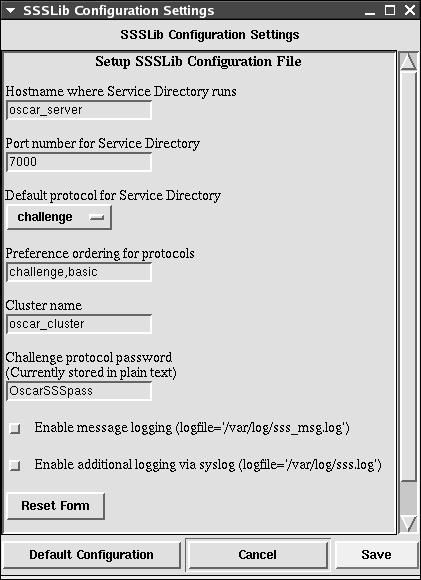
\includegraphics[scale=0.3]{figs/ConfiguratorExample}
\end{quote}



\subsubsection{post\_configure}

This is a simple \file{post\_configure} example that process the results
of the Configurator that are stored in the XML \file{.configurator.values}
file.  This reads those values to generate a configuration file
\file{/etc/ssslib.conf}.

\begin{scriptsize}
\begin{verbatim}
  #!/usr/bin/env perl
  # 'post_configure' -- reads Configurator result to setup '/etc/ssslib.conf'

  use XML::Simple;
  use Carp;

  my @fields = (sd_host, sd_port, sd_protocol, prefs, cluster, password, 
                msg_log, syslog_sss);
  my $conf     = ">/etc/ssslib.conf";
  my $xml_data = "$ENV{OSCAR_PACKAGE_HOME}/.configurator.values";


  my $ref = XMLin($xml_data) or croak("Error: unable to open ($xml_data)");
  open(CONF, $conf) or croak("Error: unable to open ($conf)\n");

  print CONF "# SSSLib configuration file\n# Generated by OSCAR\n\n";
  foreach $key  (@fields) {
          if( defined($ref->{"$key"}) ) {
                  print CONF $key, "=", $ref->{$key}, "\n";
          }
  }
  print CONF "\n";

  close(CONF);
\end{verbatim}
\end{scriptsize}

There is one important issue with multiline $<$select$>$ elements.  If the
user selects only one $<$option$>$, XMLin() in its basic form above will
return the value for the $<$select$>$ element as a SCALAR.  But if the user
selects multiple $<$option$>$s, XMLin() will return the value as an ARRAY.
To handle this case you have two options:

\begin{enumerate}
\item Use the Perl function \texttt{ref()} to determine if each hash value is
an ARRAY or a SCALAR and handle it appropriately.  
\item Call XMLin as \texttt{XMLin(FILENAME, forcearray => '1')}.  This will
force every hash value to be an array.  Thus, you can either iterate through
all hash values, or you can access the 0th element of the hash value for
those inputs you know will have only one value.
\end{enumerate}



% TJN: Finish this section...
\subsection{post\_clients}

This is an example taken from C3 that builds the \file{/etc/c3.conf} using
the information that was obtained after the nodes of the cluster have been
defined. 
\begin{scriptsize}
\begin{verbatim}
#!/usr/bin/perl
# 'post_clients' -- generate the C3 configuration file '/etc/c3.conf'

use strict;
use Carp;
use lib '/usr/lib/systeminstaller';
use SystemInstaller::Machine;
use Data::Dumper;

my $image = shift;

my $c3_conf = "/etc/c3.conf";

my $hostname = `hostname`;
chomp($hostname);

my %hash = get_machine_listing($image);

open(OUT,">$c3_conf") or croak("Couldn't open $c3_conf");
print OUT "cluster oscar_cluster {\n";
print OUT "\t$hostname\n";
my $firstkey = 1;
foreach my $key (sortnodes( keys %hash )) {
    if ($firstkey)
      {
        $hash{$key}->{HOST} =~ /([a-zA-Z_\-]+)(\d*)/;
        print OUT "\tdead remove_line_for_0-indexing\n" if 
          (defined($2) && ($2 != 0));
        $firstkey = 0;
      }
    print OUT "\t", $hash{$key}->{HOST}, "\n";
}
print OUT "}\n";
close(OUT);

# Use Schwartzian transform to sort node names alphabetically and numerically.
# Names w/o numeric suffix preceed those with numeric suffix.
sub sortnodes(@) {
	return map { $_->[0] }
	       sort { $a->[1] cmp $b->[1] || ($a->[2]||-1) <=> ($b->[2]||-1) }
	       map { [$_, /^([\D]+)([\d]*)$/] }
	       @_;
}
\end{verbatim}
\end{scriptsize}


\subsection{post\_install}

These two examples show two very simple examples of OSCAR packages that are
using this final phase script.  The OPIUM package is used to synchronize
system files across the cluster, e.g., account files like '/etc/passwd',
etc.  It takes a simple option to \cmd{--force} synchronization once all
nodes have been built since the account information is not stored in the
image that is used to build the machines.

\begin{scriptsize}
\begin{verbatim}
    #!/bin/sh
    /opt/opium/bin/sync_users --force
\end{verbatim}
\end{scriptsize}


\noindent The other package example making use of \file{post\_install} is the
NTP configuration package.  It uses a C3 parallel execution command to
restart the NTP daemon on all nodes of the cluster.

\begin{scriptsize}
\begin{verbatim}
    #!/bin/bash
    # Post install action to restart ntpds.  This is necessary because when the
    # node is booting for the first time, other nodes are sometimes building,
    # causing network saturation.  This causes the ntpd to give up and try
    # later.
  
    . /etc/profile
    cexec /etc/init.d/ntpd restart
\end{verbatim}
\end{scriptsize}



%-------------------------------------------------------------
% Section: OSCAR Package Downloader
% (This is from Jeff Squyres, taken from OLS'03 paper)
%-------------------------------------------------------------
%---------------------------------------------------------------------------
% $Id: opd.tex,v 1.2 2003/09/09 06:21:17 naughtont Exp $
%
% This section is from Jeff Squyres' section of the OLS'03 paper.
%
%  Ottawa Linux Symposium 2003 (OLS'03) Paper
%  July 23-26, 2003,  Ottawa Canada
%  http://www.linuxsymposium.org/2003/
%
% Information on the OSCAR package downloader.
%
%---------------------------------------------------------------------------


\section{OSCAR Package Downloader (OPD)}
\label{sect:opd}

The OSCAR Package Downloader (OPD) provides the capability to download
and install OSCAR software from remote package repositories.  A
package repository is simply an FTP or web site.  Given the ubiquitous
access to FTP and web servers, any organization can host their own
OSCAR package repository and publish their packages on it.  There is
no central repository; the OPD network was designed to be distributed
such that no central authority is required to publish OSCAR packages.
%
Although the OPD client program downloads an initial list of
repositories from the OSCAR Working Group web site,\footnote{The
  centralized repository list is maintained by the OSCAR working
  group.  Upon request, the list maintainers will add most repository
  sites.} arbitrary repository sites can be listed on the OPD command
line.

Since package repositories are FTP or web sites, any traditional FTP
client or web browser can also be used to obtain OSCAR packages.  Most
users prefer to use the OPD client itself, however, because it
provides additional functionality over that provided by traditional
clients.  OPD offers two interfaces: a simple menu-based mechanism
suitable for interactive use and a command-line interface suitable for
use by higher-level tools (or automated scripts).

Partially inspired by the Comprehensive Perl Archive Network (CPAN),
OPD provides the following high-level capabilities:
%
\begin{itemize}
\item Automating access to a central list of repositories
\item Browsing packages available at each repository
\item Providing detailed information about packages
\item Downloading, verifying, and extracting packages
\end{itemize}
%
While the job that OPD performs is actually fairly simple and could be
performed manually, having an automated tool for these functions
provides ease of use for the end-user, performs multiple checks to
ensure that downloaded and extracted properly, and lays the groundwork
for higher-level OSCAR package/retrieval tools.



%-------------------------------------------------------------
% Section: OSCAR Database (ODA)
%-------------------------------------------------------------
% $Id: oda.tex,v 1.1 2003/09/26 06:52:32 naughtont Exp $


\section{OSCAR Database (ODA)}
\label{sect:oda}

The database used in OSCAR is called ODA.  The information about software
packages and cluster nodes is stored in the database.  There is both a
command-line (\cmd{oda}) and Perl (\file{oda}) interface.  There are several
``shortcuts'' defined to perform queries and mask the underlying data
representation.  The current DB engine is MySQL.  See ODA(1), ODA(3pm).

\begin{verse}
    {\bfseries Notice:} More information should be added to this section.
	However, only a few packages are currently using ODA and are relatively
	sophisticated.
\end{verse}



%-------------------------------------------------------------
% Section: OSCAR Configurator
%-------------------------------------------------------------
% $Id: configurator.tex,v 1.3 2003/10/01 22:44:07 naughtont Exp $
%
% "Configurator HOWTO" (LaTeX-ified for inclusion w/ the Pkg howto)
%  - The details the usage and syntax for working with the OSCAR Configurator.
%


\section{OSCAR Configurator}
\label{sect:configurator}

This section provides details on the syntax and usage of the OSCAR
Configurator. 

\subsubsection*{Writing the \file{configurator.html} File}

To present configuration options to the user, the Configurator uses
a simple HTML \textbf{Form}. While the basics of writing HTML files
and HTML forms are discussed in detail in many books and online tutorials,
this section seeks to describe the HTML form tags available to a package
maintainer and how to use those tags to get information from the user.

Many of the basic HTML tags are supported in the OSCAR Configurator,
including:

\begin{itemize}
	\item various fonts and headers 
	\item line and paragraph breaks 
	\item horizontal (ruler) lines 
	\item centered text 
	\item images (GIFs and JPEGs) 
\end{itemize}
There is also a decent assortment of HTML Form tags such as:

\begin{itemize}
	\item input fields
	\item checkboxes
	\item radio buttons
	\item single- and multi-selection lists
	\item text boxes 
\end{itemize}
All of the available tags are described in detail in below.  There are some
HTML tags that are NOT allowed in a configuration file.  In particular, you
may \textbf{not} use:
%
\begin{description}

	\item[\xmltag{A HREF}] - A hypertext link to other places on the web.
	We don't want the user going off to another web page.

	\item[\xmltag{TABLE}, \xmltag{TR}, \xmltag{TD}] - While tables are
	parsed in without difficulty, they are not rendered as true talbes.
	Better to use \xmltag{PRE} (preformatted text) for this purpose.

	\item[\xmltag{ISINDEX}] - The document cannot be searchable.

	\item[\xmltag{SUBMIT}, \xmltag{BUTTON}, \& \xmltag{IMAGE}] - The
	Configurator has its own button to submit the values of the form to the
	program, so these elements are unnecessary.

	\item[\xmltag{FILE}] - The user is not allowed to upload a file. 

\end{description}
%
If any of these tags are present in your HTML document, they are removed
prior to rendering so that your document will appear without the offending
tags.


\subsubsection*{A Basic HTML Form Document}

Since all of the configuration input from a user appears in an HTML Form,
the minimum useful configuration file contains \xmltag{form} and
\xmltag{/form} tags. Between these two tags, the package maintainer adds
\xmltag{input} tags to get input from the user. For example, if all you
want from the user is his name, your configuration file might be as
follows:

\begin{footnotesize}
\begin{verbatim}
     <form>
     Enter your name: <input name="username">
     </form>
\end{verbatim}
\end{footnotesize}

The resulting output would look like this:

~


\includegraphics[scale=0.5]{figs/EnterYourName}


~


If you are HTML savvy, you may notice a few things missing from this
example. Specifically, we omitted the main \xmltag{html}...\xmltag{/html}
tags, and the \xmltag{head}\xmltag{/head} and \xmltag{body}\xmltag{/body}
tags. For basic configuration files, these tags are optional. You may use
them if you like (and some browsers would bonk if they were absent), but
they are not required.  Also, there are no attributes for the \xmltag{form}
tag. This is because the Configurator knows the action to take when the
user saves the values, so no {}``action'' label is needed. Also, there can
be only one pair of \xmltag{form}\xmltag{/form} tags in the configuration
file, so there is no need for the {}``name'' label.


\subsubsection*{A More Complete HTML Form}

A typical HTML document consists of at least two separate sections,
a {}``head'' and a {}``body''. The most important element of the
{}``head'' is the \xmltag{title}...\xmltag{/title} tag. This sets the title of
the window and also acts as the text for the header of the configuration
window. If you omit this tag or leave the value blank, it defaults
to {}``Configuration''.

The body is where the main part of the HTML document is stored. It
includes both the Form and any other {}``standard'' HTML elements
you want to display. Many of these elements can appear inside or outside
of the Form, so it is sometimes easiest to have a configuration form
that looks like this:

\begin{footnotesize}
\begin{verbatim}
     <html>
       <head>
         <title>The Title Of Your Configuration Form<title>
       </head>

       <body> 
         <form> 
           All of your main HTML configuration goes here.
         </form> 
       </body> 
     </html>
\end{verbatim}
\end{footnotesize}

In HTML files, whitespace (including carriage returns) are usually
compacted to a single space. So in the above example, the indentation
and line spacing are shown simply to make the example easier to read.
We could just have easily put everything on a single line and the
output would be the same. This is important to know since if you want
a true line break (say between paragraphs), you have to explicitly
tell HTML by using the \xmltag{p} (paragraph) tag. Also, the case of the
tags is unimportant, so you could also use all uppercase letters for
your tags if you find that to be more readable.


\subsubsection*{Basic (non-form) HTML Tags}

There are many HTML tags which can be displayed by the Configurator
that don't need to be in the form, but will be useful anyway. The
function of each of these tags are not listed here. There are plenty
of HTML reference books and online tutorials available. Use your favorite
search engine and do a search on {}``HTML tutorial'' to get a big
listing.


\subsubsection*{HTML Form Tags}

The main tags that you will need for your configuration file are \xmltag{form}
tags. These tags allow you to prompt the user for information to be
entered via text boxes, check boxes, radio buttons, selection lists,
etc. This section describes each tag in detail and provides examples.

Note that all of these tags must appear between a \xmltag{form}...\xmltag{/form}
tag pair. Otherwise your values will not get submitted correctly.

\begin{itemize}

%------ITEM------------
\item $<$input {}type=\char`\"{}text\char`\"{}
name=\char`\"{}VARIABLE\char`\"{} value=\char`\"{}INITIAL\char`\"{}
size=\char`\"{}NUMCHARS\char`\"{} maxlength=\char`\"{}MAXCHARS\char`\"{}$>$ 


A \textit{text} element is a single line text input field in which
the user can enter text. If you do not specify \textbf{type=''text''},
then the \xmltag{input} defaults to this type of text input field. Of the
various attributes, only \textbf{name} is required. The \textbf{name}
attribute designates the variable name for the data entered by the
user. If you also specify the \textbf{value} attribute, that text
appears in the text input field when it first appears. The \textbf{size}
and \textbf{maxlength} attributes designate the number of characters
that appear in the text box and the maximum length of the input text
respectively.

Example:

\begin{footnotesize}
\begin{verbatim}
     <form> 
     Enter your name: 
     <input type="text" name="username" value="johndoe" size="20" maxlength="30"> 
     </form>
\end{verbatim}
\end{footnotesize}

Output:


\begin{quote}

\includegraphics[scale=0.5]{figs/EnterYourName2}
\end{quote}
%------ITEM------------
\item $<$input type=\char`\"{}password\char`\"{} name=\char`\"{}VARIABLE\char`\"{}
value=\char`\"{}INITIAL\char`\"{} size=\char`\"{}NUMCHARS\char`\"{}
maxlength=\char`\"{}MAXCHARS\char`\"{}$>$ -


A \textit{password} element is a text input field in which each character
typed is displayed as a {*} to conceal the actual value entered. In
all other aspects, this element is the same as the \textit{text} element.

Example:

\begin{footnotesize}
\begin{verbatim}
     <form> 
     Enter your password: 
     <input type="password" name="password" value="passwd" size="10" maxlength="20"> 
     </form>
\end{verbatim}
\end{footnotesize}

Output: 

\begin{quote}

\includegraphics[scale=0.5]{figs/EnterYourPassword}
\end{quote}

%------ITEM------------
\item $<$input type=\char`\"{}checkbox\char`\"{} name=\char`\"{}VARIABLE\char`\"{}
value=\char`\"{}RETURNVALUE\char`\"{} checked$>$ - 


A \textit{checkbox} is a toggle that the user can select (switch on) or
deselect (switch off). As with all \xmltag{input} elements, the
\textbf{name} attribute is required and designates the variable name for
the value returned by the check box. Usually, {}``ON'' is returned when a
check box has been checked by the user. If you specify the \textbf{value}
attribute, that value is returned instead when the check box has been
checked by the user. You can optionally specify the \textbf{checked}
attribute to make the check box initially selected when first displayed.
Otherwise, the check box is unselected when first displayed. Any check
boxes which are not checked when the form is submitted do not get passed to
the Configurator, ie. their values will be {}``'' (the empty string).

Example:

\begin{footnotesize}
\begin{verbatim}
     <form> 
     <input type="checkbox" name="rootaccess" value="YES" checked> 
     Enable "root" access 
     </form>
\end{verbatim}
\end{footnotesize}

Output: 

\begin{quote}

\includegraphics[scale=0.5]{figs/EnableRootAccess}
\end{quote}

%------ITEM------------
\item $<$input type=\char`\"{}radio\char`\"{} name=\char`\"{}VARIABLE\char`\"{}
value=\char`\"{}RETURNVALUE\char`\"{} checked$>$ - 


A \textit{radio} element is a radio button. A set of radio buttons consists
of multiple radio buttons that all have the same \textbf{name} attribute.
Only one radio button in the set can be selected at one time. When the user
selects a button in the set, all other buttons in the set are deselected.
If one radio button in a set has the \textbf{checked} attribute, that one
is selected when the set is first displayed. Otherwise, none of the radio
buttons are selected when first displayed (which may not be the desired
functionality). As with all \xmltag{input} elements, the \textbf{name}
attribute is required and designates the variable name for the value
returned by the radio button set. All radio buttons with the same
\textbf{name} are in the same set, regardless of where they appear in the
form. The \textbf{value} attribute is the value that is returned for the
radio button set when the form is submitted.  This default to {}``ON''
which isn't very useful for a set of radio buttons, so be sure to give each
radio button its own \textbf{value}.

Example:

\begin{footnotesize}
\begin{verbatim}
     <form> 
     User type:<br> 
     <input type="radio" name="usertype" value="guest"> Guest<br> 
     <input type="radio" name="usertype" value="user" checked> User<br> 
     <input type="radio" name="usertype" value="admin"> Admin<br> 
     </form>
\end{verbatim}
\end{footnotesize}

Output: 

\begin{quote}
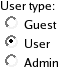
\includegraphics[scale=0.5]{figs/UserType}
\end{quote}

%------ITEM------------
\item $<$input type=\char`\"{}hidden\char`\"{} name=\char`\"{}VARIABLE\char`\"{}
value=\char`\"{}RETURNVALUE\char`\"{}$>$ - 


A \textit{hidden} element is an invisible element whose main purpose
is to contain data that the user does not enter. This data gets sent
when the form is submitted. This allows you to always pass a certain
name/value pair to the Configurator without input from the user. Both
the \textbf{name} and \textbf{value} attributes are required.

Example:

\begin{footnotesize}
\begin{verbatim}
     <form> 
     There's a hidden element here!
     <input type="hidden" name="version" value="5.23"> 
     </form>
\end{verbatim}
\end{footnotesize}

Output: 

\begin{quote}

\includegraphics[scale=0.5]{figs/HiddenElement}
\end{quote}

%------ITEM------------
\item $<$input type=\char`\"{}reset\char`\"{}
value=\char`\"{}LABEL\char`\"{}$>$
- 


When the user presses a \textit{reset} button, all elements in the
form are reset to the values that were present when the form was first
displayed. Usually, the text of this button is {}``Reset'', but
you can change this by specifying the \textbf{value} attribute.

Example:

\begin{footnotesize}
\begin{verbatim}
     <form> 
     Reset form: <input type="reset" value="Reset to Original Values">
     </form>
\end{verbatim}
\end{footnotesize}

Output: 

\begin{quote}

\includegraphics[scale=0.5]{figs/ResetForm}
\end{quote}

%------ITEM------------
\item $<$input type=\char`\"{}reset\char`\"{}
\item $<$textarea name=\char`\"{}VARIABLE\char`\"{} cols=\char`\"{}WIDTH\char`\"{}
rows=\char`\"{}HEIGHT\char`\"{} 


wrap=\char`\"{}OFF\char`\"{}|\char`\"{}HARD\char`\"{}|\char`\"{}SOFT\char`\"{}$>$Text
to display$<$/textarea$>$ - 

The \textit{textarea} tag defines a multiline input field into which the
user can enter text. As with \xmltag{input} elements, the \textbf{name}
attribute is required and designates the variable name for the text present
in the box when the form is submitted. The width and height (in terms of
characters) of the text box is given by the optional \textbf{cols} and
\textbf{rows} attributes. By default, any text entered by the user is
displayed {}``as is'' meaning that if the line input by the user is longer
than the width of the text box, the text will scroll off the screen. The
only time a new row is started is when the user types a carriage return.
This is also the behavior when you use the
\textbf{wrap=\char`\"{}OFF\char`\"{}} attribute. If you want to have the
text word wrap automatically, use the \textbf{wrap=\char`\"{}HARD\char`\"{}} 
or \textbf{wrap=\char`\"{}SOFT\char`\"{}} attribute. (In standard HTML, these
two attributes differ by whether or not the extra carriage returns
generated by word wrapping get submitted in the text or not.  For the
Configurator, these extra carriage returns are never submitted, which is
equivalent to \textbf{wrap=\char`\"{}SOFT\char`\"{}}, so using
\textbf{wrap=\char`\"{}HARD\char`\"{}} generates the same behavior.)
Between the two \xmltag{textarea}...\xmltag{/textarea} tags, you can put
optional {}``Text to display'' when the textarea is first displayed.

Example:

\begin{footnotesize}
\begin{verbatim}
     <form> 
     Comments?<br> 
     <textarea name="comments" cols=40 rows=5 wrap="SOFT"> 
     Enter your comments or suggestions here. 
     </textarea> 
     </form>
\end{verbatim}
\end{footnotesize}

Output: 

\begin{quote}
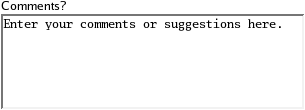
\includegraphics[scale=0.5]{figs/Comments}
\end{quote}

%------ITEM------------
\item $<$select name=\char`\"{}VARIABLE\char`\"{}
 size=\char`\"{}LISTLENGTH\char`\"{} multiple$>$ $<$option
 value=\char`\"{}OPTIONVALUE\char`\"{}$>$ $<$option
 value=\char`\"{}OPTIONVALUE\char`\"{} selected$>$ ... $<$/select$>$ - 


The \textit{select} and \textit{option} tags define a selection list.
A selection list displays a list of options from which the user can
select one (or more) items. If the \textbf{multiple} attribute is
present, the user can select multiple items from the list at a time.
Otherwise, only a single item can be selected at a time. As with \textbf{input}
elements, the \textbf{name} attribute is required and designates the
variable name for the value(s) selected in the list when the form
is submitted. The optional \textbf{size} attribute indicates how many
items are presented in the box before scrolling is necessary. This
defaults to {}``10''. If you set \textbf{size} to {}``1'' and
do not set the \textbf{multiple} attribute, you get a single element
drop-down list.

To actually put items in the selection list, you use the \textit{option}
tag followed by the text you wish to appear in the list. You can make
that option selected when the list is initially displayed by using
the \textbf{selected} attribute. By default, the value that gets returned
to the Configurator when an item is selected is the actual text of
the item in the list. You can override this behavior by using the
optional \textbf{value} attribute. When you set this value, it gets
returned when that item in the list is selected.

Example:

\begin{footnotesize}
\begin{verbatim}
     <form> 
     Select the machines to use:<br> 
     <select name="machinelist" size=5 multiple> 
     <option selected>oscar1 
     <option>oscar2 
     <option>oscar3 
     <option>oscar4 
     <option>oscar5 
     <option>oscar6 
     <option value="unlisted">unlisted machine 
     </select> 
     </form>
\end{verbatim}
\end{footnotesize}

Output: 

\begin{quote}
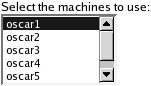
\includegraphics[scale=0.5]{figs/SelectMachine}
\end{quote}

Note: when viewing the above example in a standard HTML browser, you might
have to use the \xmltag{SHIFT} or \xmltag{CTRL} key in conjunction with
clicking the mouse to select multiple items from the list. In the
Configurator, this extra keypress is not required.

\end{itemize}



%\bibliographystyle{unsrt}
%\bibliography{./OSCAR,./CLUSTER,./OLS03}


%=============================================================
%
% **** START APPENDIX SECTIONS ****
%
%=============================================================
\newpage   %don't use newpage to keep formatting.."sane" for now
\appendix


%-------------------------------------------------------------
% Appendix: Switcher for Environment Mgmt
% (This is from Jeff Squyres, taken from OLS'03 paper)
%-------------------------------------------------------------
%---------------------------------------------------------------------------
% $Id: env-switcher.tex,v 1.1 2003/09/26 06:52:32 naughtont Exp $
% (FROM: env-switcher.tex,v 1.4 2003/05/18 02:48:28 tjn)
%
%  Ottawa Linux Symposium 2003 (OLS'03) Paper
%  July 23-26, 2003,  Ottawa Canada
%  http://www.linuxsymposium.org/2003/
%
% Information on the env-switcher package.
%
%---------------------------------------------------------------------------
%
% TJN: I have removed the cites{} since we don't do a Reference section.
%
% TJN: (TODO) Add comments on how to install a switcher module & create
%      a switcher RPM.
%

\section{Env-Switcher}
\label{sect:switcher}

Managing the shell environment -- both at the system-wide level as
well as on a per-user basis -- has historically been a daunting task.
For cluster-wide applications, system administrations typically need
to provide custom, shell-defendant startup scripts that, create and/or
augment \envvar{PATH}, \envvar{LD\_\-LIBRARY\_\-PATH}, and
\envvar{MANPAGE} environment variables.
%
Alternatively, users could hand-edit their ``dot'' files (e.g.,
\file{\$HOME/.profile}, \file{\$HOME/.bashrc}, and/or
\file{\$HOME/.cshrc}) to create/augment the environment as necessary.
%
Both approaches, while functional and workable, typically lead to
human error -- sometimes with disastrous results, such as users being
unable to login due to errors in their ``dot'' files.

Instead of these models, OSCAR provides the \package{env-switcher}
OSCAR package. \package{env-switcher} forms the basis for simplified
environment management in OSCAR clusters by providing a thin layer on
top of the Environment Modules
%package~\cite{furlani91:_modul,furlani96:_abstr_yours_with_modul}.
package (Furlani \& Osel).
Environment Modules provide an efficient, shell-agnostic method of
manipulating the environment.  Basic primitives are provided for
actions such as: add a directory to a \envvar{PATH}-like environment
variables, displaying basic information about a package, and setting
arbitrary environment variables.  For example, a module file for
setting up a given application may include directives such as:
%
\begin{verbatim}
  setenv FOO_OUTPUT $HOME/results
  append-path PATH /opt/foo-1.2.3/bin
  append-path MANPATH /opt/foo-1.2.3/man
\end{verbatim}
% Stupid emacs mode: $
%
The \package{env-switcher} package installs and configures the base
Modules package and creates two types of modules: those that are
unconditionally loaded, and those that are subject to system- and
user-level defaults.

Many OSCAR packages use the unconditional modules to append the
\envvar{PATH}, set arbitrary environment variables, etc.  Hence, all
users automatically have these settings applied to their environment
(regardless of their shell) and guarantee to have them executed even
when executing on remote nodes via \cmd{rsh}/\cmd{ssh}.

Other modules are optional, or a provide one-of-many selection
methodology between multiple equivalent packages.  This allows the
system to provide a default set of applications, that optionally can
be overridden by the user ({\em without} hand-editing ``dot'' files).
%
A common example in HPC clusters is having multiple Message Passing
%Interface (MPI)~\cite{geist96:_mpi2_lyon,mpi_forum93:_mpi}
Interface (MPI)
implementations installed.  OSCAR installs both the
%LAM/MPI~\cite{burns94:_lam} and MPICH~\cite{Gropp:1996:HPI}
LAM/MPI and MPICH
implementations of MPI.  Some users prefer one over the other, or have
requirements only met by one of them.  Other users wish to use both,
switching between them frequently (perhaps for performance
comparisons).

The \package{env-switcher} package provides trivial syntax for a user
to select which MPI package to use.  The \cmd{switcher} command is
used to select which modules are loaded at shell initialization time.
For example, the following command shows a user selecting to use
LAM/MPI:
%
\begin{verbatim}
  shell$ switcher mpi = lam-6.5.9
\end{verbatim}
% Stupid emacs mode: $

\subsection{Example Switcher Module file}

This example was taken from the PVM module file, which gets loaded
unconditionally for all shells.

\begin{footnotesize}
\begin{verbatim}
# PVM modulefile for OSCAR clusters (based on LAM modulefile)

proc ModulesHelp { } {
  puts stderr "\tThis module adds PVM to the PATHand MANPATH."
  puts stderr "\tAdditionally the PVM_ROOT and PVM_ARCH are set."
}

module-whatis   "Sets up the PVM environment for an OSCAR cluster."

setenv PVM_RSH  ssh
setenv PVM_ROOT /opt/pvm
setenv PVM_ARCH LINUX

append-path MANPATH /opt/pvm/man

append-path PATH /opt/pvm/lib
append-path PATH /opt/pvm/lib/LINUX
append-path PATH /opt/pvm/bin/LINUX
\end{verbatim}
\end{footnotesize}



%-------------------------------------------------------------
% Appendix: Section w/ Table of supported XML tags
%-------------------------------------------------------------
%  $Id: pkg-xml-table.tex,v 1.1 2003/09/08 22:31:35 naughtont Exp $

% TJN: Note I'm using the "(" symbol for the \verb delimiters b/c
%      I don't believe this symbol will occur in any of the XML elements
%      or attributes.  Any other non-occuring char could be used.
%
% TJN: I need some way to convey heirarchy, currently using multi-columns
%      xml   &      &  descr... \\
%      dtd   &      &  descr... \\
%      oscar &      &  descr... \\
%            & name &  descr... \\
%
% TJN: Somehow I need to display <tag></tag>  VS. <tag/>
%      Also, certain things like <description></description> must be
%      on same line as closing multi-line text.  Need to check this out
%      I believe it's a product of using XML::Simple.
%
% TJN: Also, I need to denote optional vs. required elements

\begin{table}[htbp]
  \begin{center}
  \begin{tabular}{|l|l|l|} \hline
  {\bfseries Top-Level Tag} & {\bfseries Sub Tag} & {\bfseries Description}\\\hline
  \hline
  \verb(<?xml version="1.0"?>( & &  Opening XML Version string         \\ \hline
  %\verb(<!DOCTYPE package SYSTEM "../package.dtd">( & & DTD Include line\\\hline

  \verb(<!DOCTYPE ...>( & & Document Type Definition (DTD) Include line\\ \hline
  \verb(<oscar>(   &   & OSCAR Package Element                         \\ \hline
  \verb(<name>(    &   & Name of the software package                  \\ \hline

  %\verb(<version>( &   & Version of the software package               \\ \hline
  \verb(<version>( &   & Version of the software package           \\\cline{2-3}
     & \verb(<major>(  & Major version of the software package     \\\cline{2-3}
     & \verb(<minor>(  & Minor version of the software package     \\\cline{2-3}
     & \verb(<subversion>( & Sub-version of the software package   \\\cline{2-3}
     & \verb(<release>(    & Release number of the software package\\\cline{2-3}
     & \verb(<epoch>(      & Release number of the software package\\\hline

  \verb(<class>(   &   & Classification of package, e.g. third-party   \\ \hline
  \verb(<summary>( &   & Brief one-line description of package         \\ \hline
  \verb(<license>( &   & Software licence for the package              \\ \hline
  \verb(<group>(   &   & RPM-style software group, e.g., Application/System\\\hline
  \verb(<url>(     &   & Homepage for software package                 \\ \hline

  %\verb(<packager>(&   & OSCAR package author                         \\ \hline
  \verb(<packager>(&   & OSCAR package author                      \\\cline{2-3}
     & \verb(<name>(   & Name of package author                    \\\cline{2-3}
     & \verb(<email>(  & Email address of package author           \\\hline

  %\verb(<maintainer>(& & OSCAR package author                         \\ \hline
  \verb(<maintainer>(& & OSCAR package author                      \\\cline{2-3}
     & \verb(<name>(   & Name of package author                    \\\cline{2-3}
     & \verb(<email>(  & Email address of package author           \\\hline

  \verb(<description>(&& Brief description of the package              \\ \hline

  %\verb(<rpmlist>(&    & List RPMS included in the rpmlist             \\ \hline
  \verb(<rpmlist>(&    & List RPMS included in the rpmlist         \\\cline{2-3}
     & \verb(<filter>( & Filter applied to all RPM in list         \\\cline{2-3}
     & \verb(<rpm>(    & Name of RPM (without version)             \\\hline

  %\verb(<filter>(&     & Filter Attributes used on RPMLIST              \\\hline
  \verb(<filter>(&     & Filter Attributes used on RPMLIST            \\\cline{2-3}
     & \verb(group=(   & Attribute specifying target location for RPMS\\
     &                 & e.g., ``oscar\_server'' or ``oscar\_clients''\\\cline{2-3}
     & \verb(distribution=(& Attribute specifying supported distribution   \\
     &                 & e.g., ``redhat'', ``mandrake'', ``suse'', ``rhas''\\
     &                 & see also: \emph{lib/OSCAR/Distro.pm}              \\\cline{2-3}
     & \verb(distribution_version=(& Attribute specifying supported distribution version  \\
     &                 & e.g., ``7.3'', ``9'', ``2.1AS''                   \\\hline

  %\verb(<requires>(&   & List requirement/dependency                    \\\hline
  \verb(<requires>(&   & List requirement/dependency                \\\cline{2-3}
     & \verb(type=(    & Tag specifying type of requirement         \\
     &                 &  e.g., ``package'' (OSCAR Package),        \\
     &                 &  \emph{``rpm'' (not implemented yet)}      \\\hline

  %\verb(<package>( &   & Package specific ODA material                \\\hline 
  \verb(<package>( &    & Package specific ODA material            \\\cline{2-3}
     & \verb(<shortcut>(& ODA shortcut defined by a package            \\\hline

  \end{tabular}
  \caption{Overview of existing XML tags for OSCAR Packages} 
  \label{tab:pkg-xml-tags}
  \end{center}  
\end{table}



%-------------------------------------------------------------
% Appendix: Add information about using XML tools like 'xmllint'
%           and the DTD/Schema material.
%-------------------------------------------------------------
%\input{xml-tools.tex}

\end{document}

